\documentclass[10pt,a4paper]{book}
\usepackage[top=1in, bottom=1in, left=1in, right=1in]{geometry}
\usepackage[utf8]{inputenc}
\usepackage{amsmath}
\usepackage{amsfonts}
\usepackage{amssymb}
\usepackage{graphicx}
\usepackage[colorlinks]{hyperref}
\hypersetup{urlcolor=blue}

\author{Mart\'in Baigorria}
\title{Documentation \\ Price Risk Monitor}

\begin{document}

\maketitle

\chapter{Implied Risk Neutral Distribution Indicator}
\section{Introduction}
Option prices across strike prices provide relevant information about market expectations on the price distribution of the underlying asset. By using a slight variation of Figlewsky's method, which is described in detail in 'Estimating of the Implied Risk Neutral Density for the U.S. Market Portfolio', we were able to extract these distributions and quantify the probabilities of different price variations.

The following guide aims to explain in detail how to use and update the Soybean \& Corn Price Risk Monitor. Our script calculates these distributions automatically from option prices on futures with real-time data taken from the CME Group (Chicago Mercantile Exchange \& Chicago Board of Trade).

To understand this guide, it is highly advised you have some basic Matlab knowledge. You will also need Matlab version R2014a or higher.

\section{Methodology}
The methodology used is clearly explained in Figlewsky's paper. However, to sum up, this is the general procedure:
\begin{enumerate}
  \item Option data is extracted from the CME in JSON format\footnote{JSON: Javascript Object Notation: \url{http://json.org}}. This guarantees the robustness of our data extraction method. The data units are cents per bushel. It is fairly easy to convert it to USD per ton. For more information about unit conversions, see the 'Agricultural Commodity Metric Conversion Guide' by the CME.
  \item Option prices are transformed into the implied volatility space by using the Black-Scholes implied volatility formula.
\raggedbottom
\pagebreak
  \item The empirical volatility smile is then approximated by a quartic polynomial to allow us to capture asymmetries in the market. Our old degree two polynomial failed to capture this. The implied volatility calculated from calls and puts may be quite different even when there is data available at the same strike price, or even when you start considering strike prices that are at a higher distance from the underlying asset price. This is why a blending threshold is defined. This threshold defines the range in which volatilities are going to be blended to then fit the polinomial on a final volatility series.
  \item Once we have the volatility smile fit, data is once again transformed into the price space by using the Black-Scholes formula. Option prices are not used at once because prices of options in between strikes is not available. This way we can robustly generate prices across all strike prices.
 \item With these generated prices, a discrete approximation of the probability density and distribution is computed between the original strike price ranges. Since we can control the distance between strikes, this approximation is fairly good. This formula taken from Figlewsky is pretty straightforward to calculate, and it can easily be understood by reading pages 6, 7 and 8 of his paper.
  \item The tails of the distribution are usually not available when using data between the original strike price range. This is why we use a generalized extreme value (GEV) distribution to fit both of the tails we are missing. However, the numerical method to find the GEV parameters does not guarantee convergence.
  \item Once this procedure has been completed, we run several diagnosis tests to assure the distribution is well behaved and the results make sense. To do this, we compare the calculated contract prices based on the calculated distribution with the original prices. For example, for calls:

\begin{equation}
	C = \int_{X}^{\infty} e^{-rT} (S_T-X)f(S_T) dS_T
\end{equation}  
  
Once we compute this from discrete data, we simply calculate the present value of the payoff of the option. We then average the absolute differences between prices in a 20\% price range from the underlying price and set a rejection threshold. The rejection threshold must depend on the fact that the tail fit can fail, since you may be missing to integrate a relevant part of the density function. If no tails fail, we set a threshold for both calls and puts of 3\%. If a tail fit fails, we allow a difference of up to 5\%. 
\end{enumerate}

\raggedbottom
\pagebreak

\section{Usage}
\subsection{General Structure}
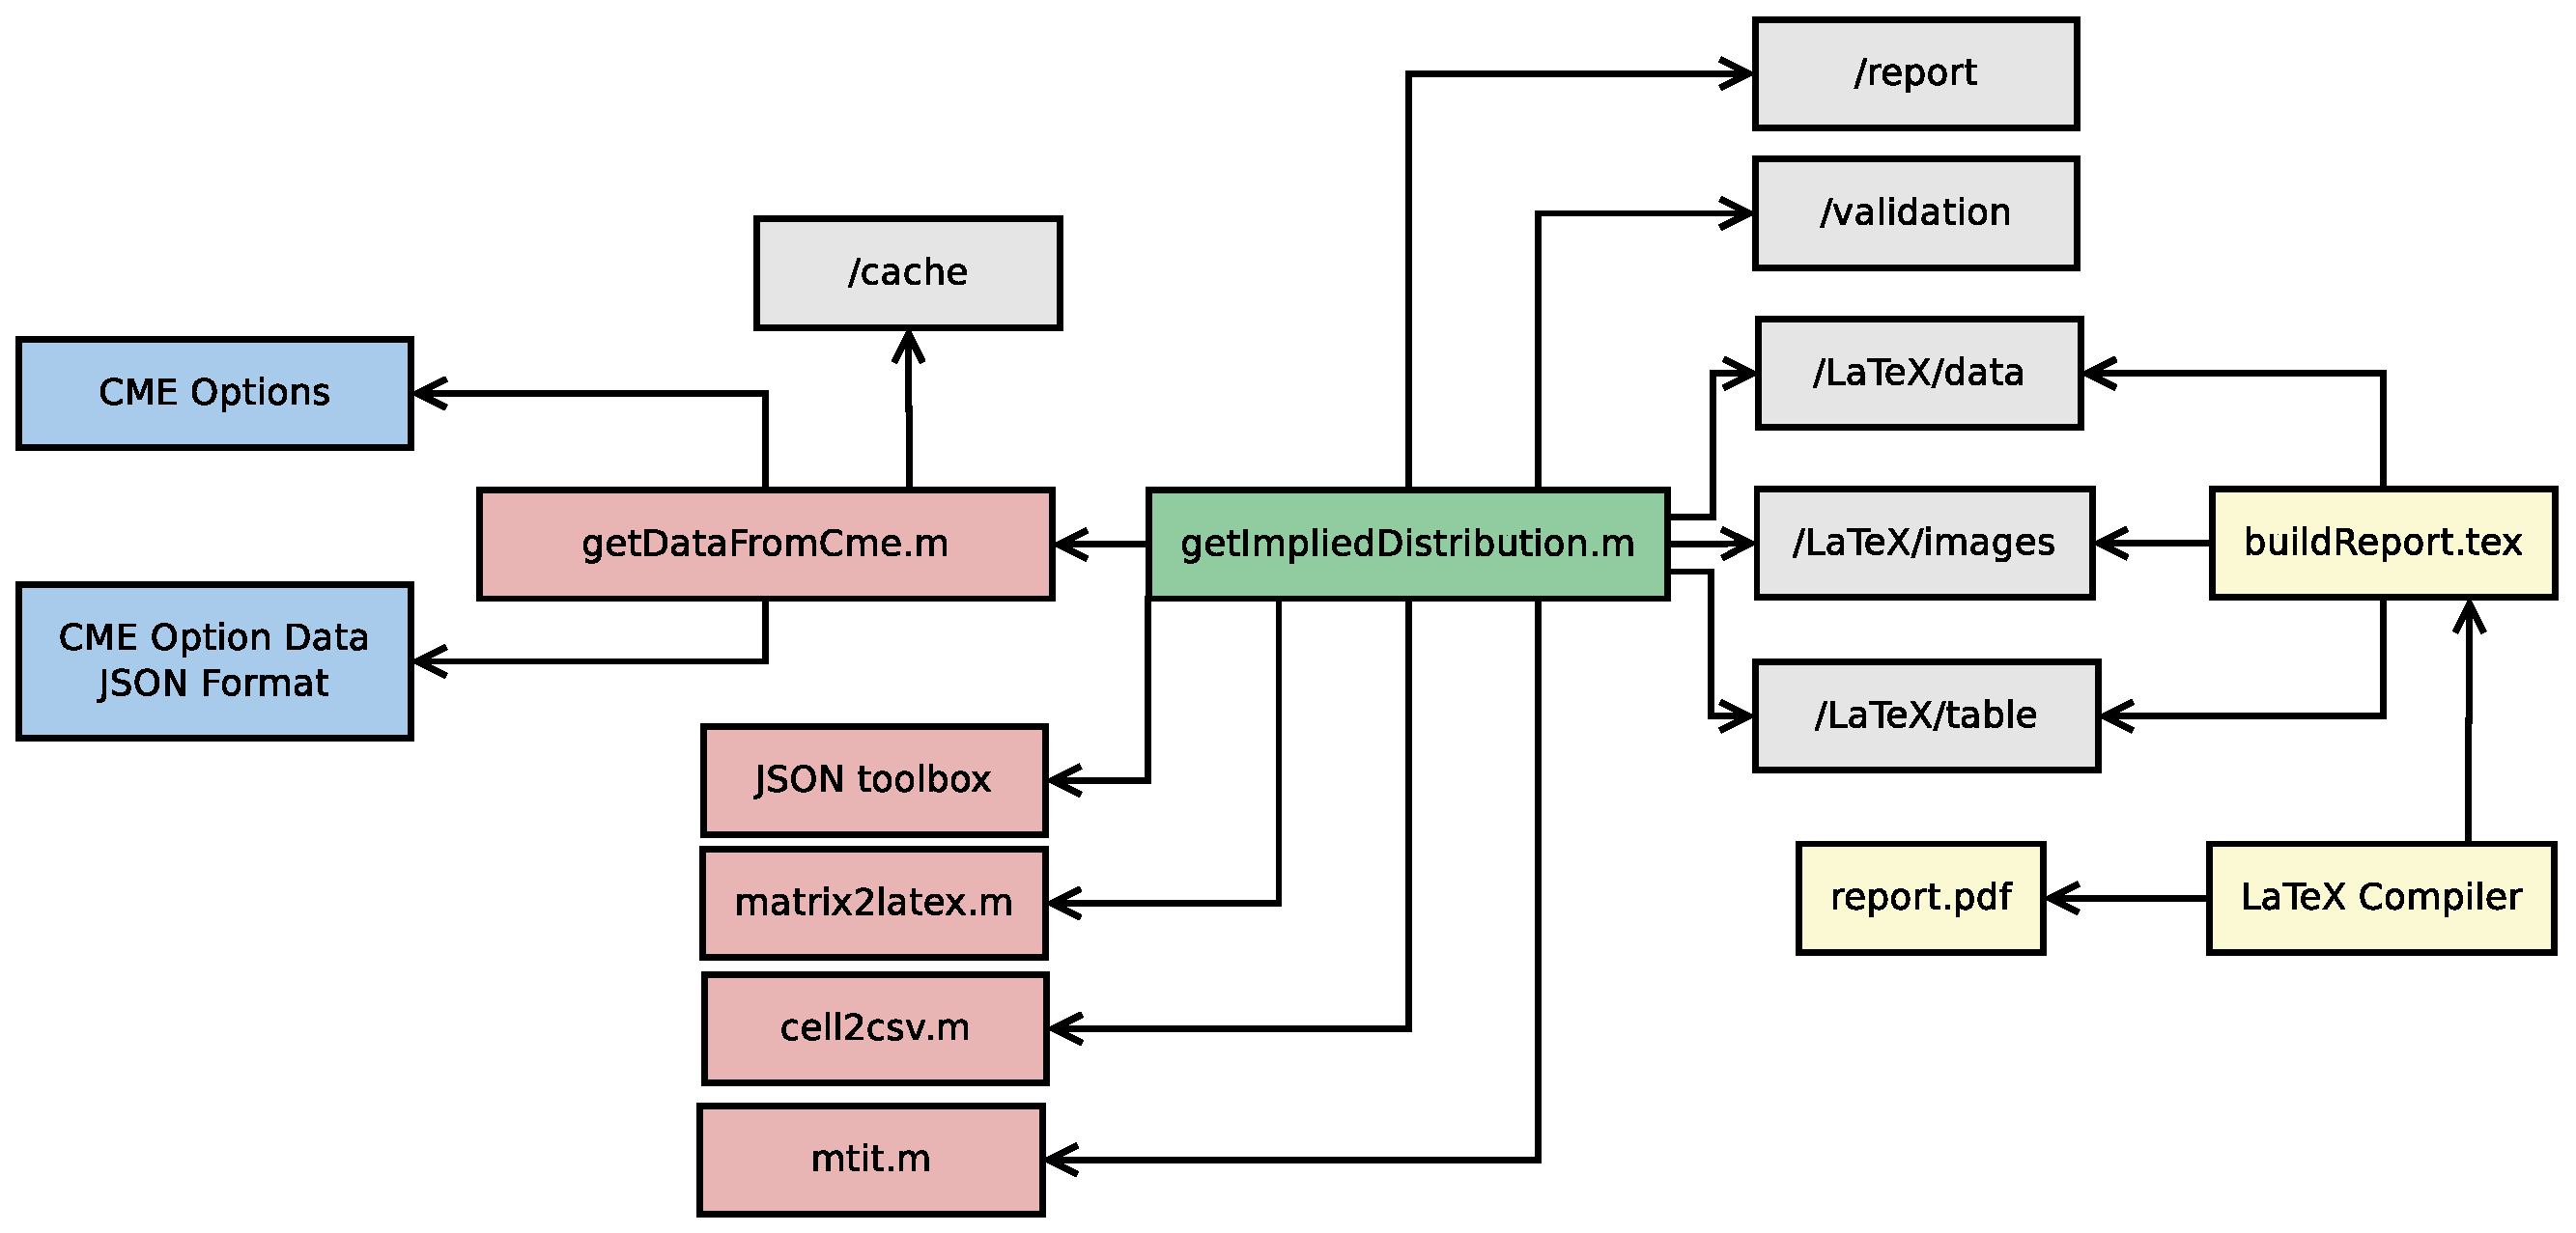
\includegraphics[width=\textwidth]{images/flow}
The diagram above aims to give a general idea about how the folders (grey) and dependencies (light red) used are structured. The main script is getImpliedDistribution.m. This script has the following dependencies:
\begin{enumerate}
  \item JSON toolbox: Allows us to load an generate JSON strings.
  \item getDataFromCme.m: Loads the option data from CME. The external resources requested are in blue. This is a bit technical and specific, but in order to request the JSON option data, we must first produce a syntactically correct request URL. This is why we must first request the main options data.
  \item matrix2latex.m: Converts Matlab matrices into latex table format.
  \item cell2csv.m: Converts a Matlab cell array into CSV.
  \item mtit.m: Allows us to add a general title to graphs with multiple subgraphs. Useful to identify graphs when we want to combine several eps files into a pdf when using gs\footnote{Ghostscript: \url{https://en.wikipedia.org/wiki/Ghostscript}}.
\end{enumerate}
Once the main script finishes running, several files are created/modified:
\begin{enumerate}
  \item The folder /validation is filled with an image that describes the whole data process for each option expiration date. The file name format is assetType-optionCode-expirationCode. This is used to validate the procedure before uploading the data to the indicator.
  \item /report is filled with images and data to easily build a report.
  \item /data, /images and /tables are filled with text and image files used to generate good looking and customizable pdf reports. These are generated via LaTeX.
  \item /cache is a folder used by getDataFromCme.m to store JSON data. Every time we try to download data from the CME, the script will first try to see if we have already downloaded it by checking this folder.
  \item loadData.csv is created in the main folder. This is a csv file that must be loaded with the delimiter ';'. This is explained in detail in the following sections.
  \item history.csv, a csv file that stores the data that is retrieved and calculated every day.
\end{enumerate}

\raggedbottom
\pagebreak

\subsection{Parameters}
The main script getImpliedDistribution.m has several parameters that may be edited:
\begin{enumerate}
  \item selectUnit (deprecated)
    \begin{itemize}
    \item 1 - Metric Tons
    \item 2 - Bushels
    \end{itemize}
  \item selectPrice: There are many prices which can be used to calculate the implied distribution.
    \begin{itemize}
    \item 2 - Best Bid
    \item 3 - Best Offer
    \item 4 - Average Price
    \item 5 - Prior Settle
    \end{itemize}
Prior settle offers more available data across strikes. The script is usually more stable when using this option. However, for real time estimates using the average price is advised.
  \item R: Risk-free rate. We will usually use the LIBOR.
  \item blendThreshold: Threshold to define which range of IVs is going to be blended.
  \item dS: Used for numerical integration.
  \item fitDegree: Degree of the polynomial we fit to the volatility smile. Even if degree two polynomials work, they fail to capture asymmetries in the distribution. This is why we tend to use a quartic polynomial.
  \item leftDif \& rightDif: These parameters are used to define the borders for the GEV fit. For more information, read pages 17-20 of Figlewsky's paper.
  \item priceRange\_*: Allows you to set the values to compute the probability chance table.
  \item dataVerification: Enables verification files.
  \item pricesCheck: Enables price checks.
\end{enumerate}

\subsection{Guide}
In first place, you must open getImpliedDistribution.m in Matlab and run the script. The following should show up in the command window.
\\ \\
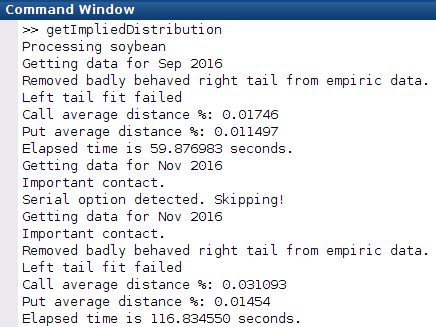
\includegraphics[scale=0.6]{images/commandWindow}

Once the script finishes loading, /validation will be full of images (one for every option loaded) and the file loadData.csv will be created in the main folder. Let us first display a sample file created in /validation:

\begin{center}
  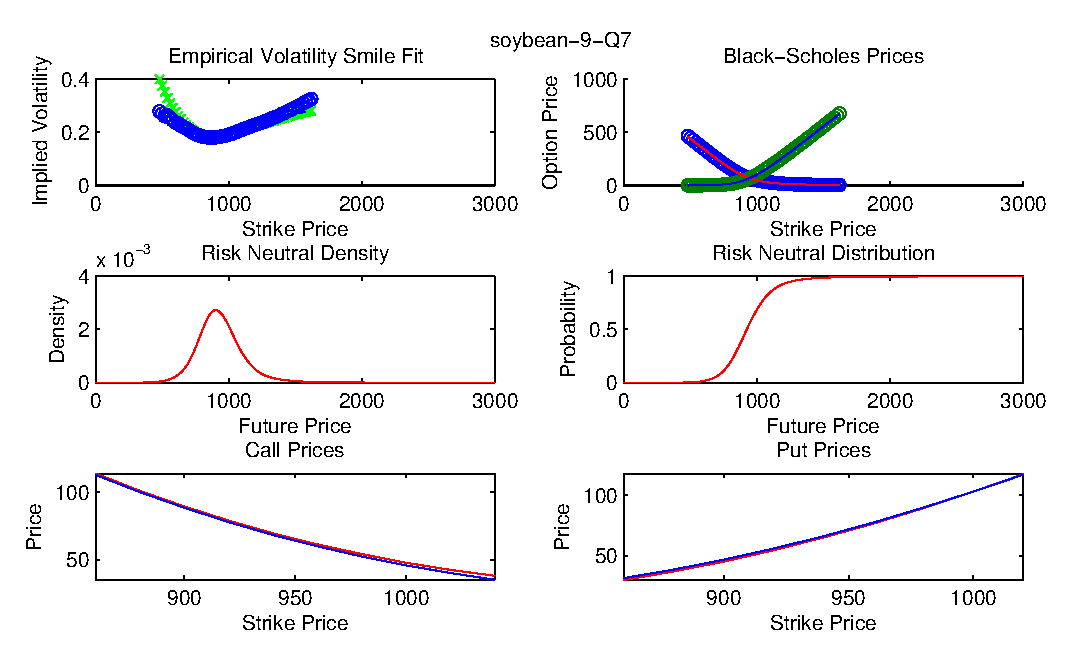
\includegraphics[scale=0.75]{images/visualValidation}
\end{center}

As you can see, the volatility smile is convex, the density and the distribution behave properly. The lower row in the graph plots both empiric and calculated call and put prices. The graph on the left corresponds to the calls and the graph on the right corresponds to the puts. In this particular example, you can see both price series match pretty well. These series are supposed to match if we are going to say our results are valid. The automatic diagnostic tests are based on these series. Only the contracts that pass this diagnostic and the important contracts will be then loaded into loadData.csv.

%When we go outside the original price range (from around 250 to 550), the Black-Scholes prices on the second graph may behave in a strange way. This is because the volatility effect beats the strike price effect on the price of the option. These generated prices are not used anyway. This particular graph looks fairly good.

loadData.csv is a file that stores the data of all the contracts that passed the diagnostic tests and the important contracts. We save important contracts even if they do not pass the validation threshold, so it's up to the analyst to decide if those results are valid by using the validation graphs. In general they all pass the tests, but sometimes they fail by a small margin.

Once we verify all graphs and select the ones we do not want to load into the indicator by deleting its corresponding row in the csv file, we must load the csv data into the web interface of the indicator. We chose '\textbf{;}' as the data delimiter, because the spreadsheet will also have JSON data that also uses a comma. This means that if we used the default delimiter '\textbf{,}', we would split the data in more columns than what we originally intended to.

In Open Office, it would look like this:

\begin{center}
  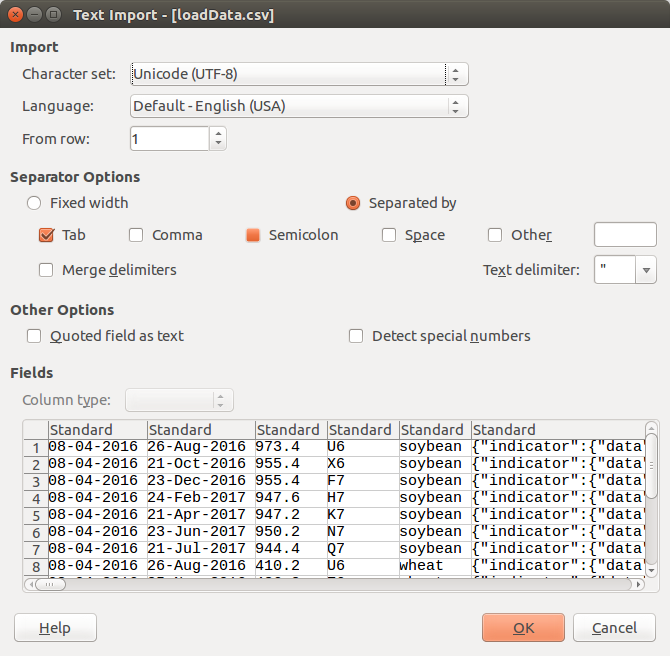
\includegraphics[scale=0.40]{images/delimiter}
\end{center}

\begin{center}
  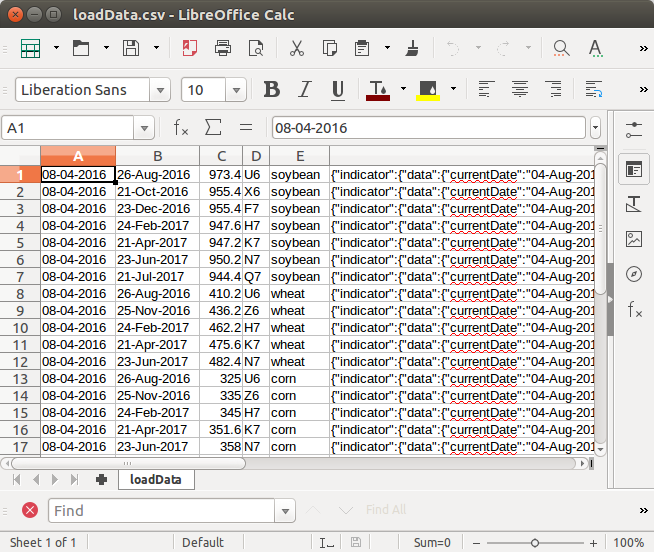
\includegraphics[scale=0.40]{images/loadData}
\end{center}

Copy the options you want to load into the indicator, and open the following 
\href{https://docs.google.com/spreadsheets/d/18GAQ\_Rk8IFyiwPd2wjh\_4VAdpe0bmxBvUxWXxIIhoZ4/edit\#gid=0}{Google Spreadsheet}. We use Google Spreadsheets to load the data to avoid having to use any type of SQL database or anything that requires any type of server/extra infrastructure. Paste the options into the bottom of the spreadsheet, it should then look like this.

\begin{center}
  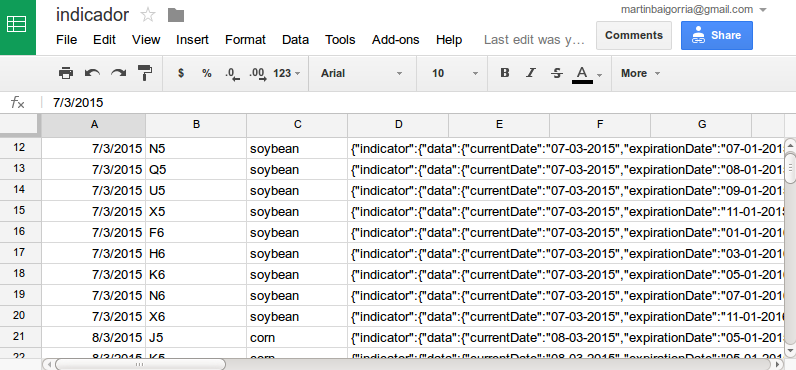
\includegraphics[scale=0.5]{images/spreadsheet}
\end{center}

This will automatically load all the data into the user interface. Note that in order to modify the spreadsheet, you must have write access.

\pagebreak

The indicator will finally look like this:

\begin{center}
  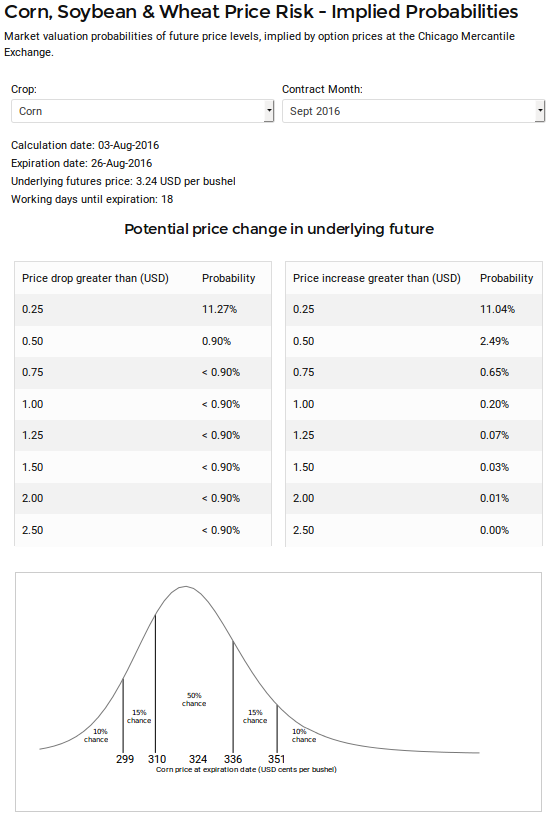
\includegraphics[scale=0.7]{images/indicator}
\end{center}

Once of the columns we loaded in the spreadsheet might not make much sense to you. That value in particular is a JSON representation of the option data, the density and the probability tables. It's a great way to store and load data fast and easily with Javascript. The indicator uses the Google Spreadsheet API for the data management and D3 library for the density visualization.

\pagebreak

\subsection{Report Generation}
Once you have run getImpliedDistribution.m, you can easily build a pdf report by running the file buildReport.tex with a LaTeX compiler (for example, \href{www.miktex.org}{Miktex}, which is usually used by \href{http://www.xm1math.net/texmaker/}{Texmaker}). Select the options you want to display in the report by copy-pasting the code shown there. Change the numeric values of includegraphics and input. If you do something wrong, you will easily notice since the report will show repeated graphs and/or data.

\subsection{Shell script}

The shell script run.sh runs in UNIX operating systems only and does the following:

\begin{itemize}
  \item Runs getImpliedDistribution.m
  \item Opens loadData.csv in Open Office.
  \item Opens a new Firefox tab on the Google Spreadsheets website to load the data.
  \item Uses Ghostscript to unify all .eps files in /validation, and then deletes the files. It is really unconfortable to open every eps file one by one to do a quick validation, this is why we unify them.
\end{itemize}

It should be fairly easy to write the corresponding commands for it to work on Windows. However, looks like when you run Matlab in interactive mode, the resolution of the /report files generated change. There are also some language encoding problems. This is why you should run the script straight from Matlab if you really need these graphs, since it looks like this is a Matlab bug.

\section{Final remarks}
\subsection{Future improvements}
\begin{enumerate}
\item The GEV fit can be improved by using other type of numerical solvers for the GEV distribution, maybe finding a native way to fit it instead of having to write the whole formula.
\item The automatic data retrieval module may be improved to be able to get data from any type of option from CME. Right now it needs some minor tweaks to work for a new option, and it cannot be generalized.
\end{enumerate}

\subsection{Other comments}
\begin{enumerate}
  \item CME last settle data usually has consecutive repeated values. This is why we run two loops, one for calls and one for puts, to clean these values and set them to NaN.
  \item How volatility blending works?
  We first go from the price space to the volatility space on both calls and puts. For a same strike, it is possible to have two different volatility values. This is why we need some sort of criteria to unify the datapoints. We will define a 'blending range' as the range around the underlying price we weight both volatilities into one value. This range is (underlyingPrice - blendThreshold; underylingPrice + blendThreshold). blendThreshold is a parameter that can be changed, we set it to 30. For values below underlyingPrice - blendThreshold, we pick the out of the money volatility for puts. For values above underlyingPrice + blendThrehold we pick the values for out of the money calls.
  Once we have this, we pick a polynomial of some degree. The degree can be controlled with the parameter fitDegree.
  \item This process does not guarantee us we will have complete information about the tails of the pdf. This is why we fit a GEV distribution, which has three values to obtain numerically for each tail. These are $\alpha$, $\alpha_0$ and $\alpha_1$. To explain why we have three variables, let's try to understand the intuition. Imagine you stop having data about the right tail at a strike price of 100. The GEV needs two points to stick itself to the empirical pdf plus a restriction that guarantees us that the tail will have a correct integral. $\alpha$ is how much the tail must integrate. We decided to make this a dynamic value depending on the data. We take the most extreme data point to get the max (min) value of the cdf. This will give us one of the points we will need for the GEV. From there, we use the values rightDif or leftDif (around 0.03) to get the other value required. This means we only need to manually set one value instead of three. The first point we chose has the restriction that it accumulates 0.05 or less (less depends on data). In general, this doesn't affect our probability tables, eventually just the martingale conditions.
  \item Sometimes we do not have enough data to quantify the probability of certain outcomes. In general, this happens when we have a distribution with a low variance. This is why sometimes we simply bound these probabilities. You can see it in the example tables above, where the probability of a price drop higher than 0.75 cents per bushel is bounded by $<$ 0.90\%.
  \item All martingale conditions are calculated on the new pdf. If a tail fit fails, we calculate it based on the pdf available.
  \item Any chances to the user interface will probably have to be implemented by changing the HTML of the indicator and the Javascript file indicator.js. We suggest you back up everything before doing such a change.
\end{enumerate}

\subsection{Useful links}
\begin{enumerate}
\item \href{http://faculty.baruch.cuny.edu/lwu/890/FiglewskiRND_draft7.pdf}{Estimating the Implied Risk Neutral Density for the U.S. Market Portfolio by Stephen Figlewski}
\item \href{https://docs.google.com/spreadsheets/d/18GAQ_Rk8IFyiwPd2wjh_4VAdpe0bmxBvUxWXxIIhoZ4/edit#gid=0}{Google Spreadsheet Database}
\item \href{www.cmegroup.com/trading/agricultural/grain-and-oilseed/soybean_quotes_globex_options.html}{Soybean Quotes}
\item \href{http://www.cmegroup.com/trading/agricultural/grain-and-oilseed/soybean_contractSpecs_options.html}{Soybean Contract Specs}
\item \href{http://www.cmegroup.com/trading/agricultural/grain-and-oilseed/soybean_product_calendar_options.html}{Soybean Contract Calendar}
\item \href{http://www.cmegroup.com/trading/agricultural/grain-and-oilseed/corn_quotes_globex_options.html}{Corn Quotes}
\item \href{http://www.cmegroup.com/trading/agricultural/grain-and-oilseed/corn_quotes_globex_options.html}{Corn Contract Specs}
\item \href{http://www.cmegroup.com/trading/agricultural/grain-and-oilseed/corn_product_calendar_options.html}{Corn Contract Calendar}
\item \href{http://www.crbtrader.com/support/symbology.asp}{Month Code Symbology}
\item \href{http://www.cmegroup.com/trading/agricultural/files/AC-225_MetricGuide.pdf}{Agricultural Commodity Metric Conversion Guide}
\end{enumerate}

\end{document}